\documentclass[conference]{IEEEtran}
\usepackage{cite}
\usepackage{amsmath,amssymb,amsfonts}
\usepackage{graphicx}
\usepackage{booktabs}
\usepackage{url}

\begin{document}

\title{DWT-DCT Watermark Design Under AI-Based Image Enhancement}

\author{\IEEEauthorblockN{Shiva Tan}
\IEEEauthorblockA{Independent Researcher\\
shivatan21@gmail.com}}

\maketitle

\begin{abstract}
Classical DWT-DCT image watermarking has traditionally been evaluated
against compression, filtering, and noise-based attacks, where watermark
degradation is closely coupled with visible image distortion. We
investigate whether AI-based image enhancement introduces a fundamentally
different robustness challenge. Across 100 images from the Kodak and
TAMPERE17 datasets at four embedding strengths, Real-ESRGAN reduces mean
normalized correlation (NC) from 0.999 to 0.795 while maintaining the
highest perceptual quality among all evaluated attacks (SSIM 0.906);
ESPCN, sharing the identical $4\times$ upscale and Lanczos downscale
pipeline, preserves watermark recovery (NC 0.999), indicating that
degradation arises from the learned reconstruction rather than resampling
alone. Coefficient-level analysis across 102,400 DCT blocks reveals
markedly different perturbation profiles for Real-ESRGAN and JPEG
compression, with strongly opposing coefficient rankings (Spearman
$\rho = -0.716$ vs.\ empirically measured JPEG damage; $\rho = -0.907$
vs.\ the JPEG quantization table). An exhaustive search over 1,953
coefficient pairs identifies a 37-pair Pareto frontier and establishes
that no pair simultaneously optimizes robustness to both attacks. A
three-pair head-to-head validation across all 100 images at four
embedding strengths confirms strongly attack-specific ordering: the
high-frequency pair $(7,5)/(7,7)$ achieves the highest Real-ESRGAN NC
(0.831 vs.\ 0.783 for the standard pair), while the analytically
balanced pair $(2,3)/(3,2)$ achieves the highest JPEG NC (0.998) but
the lowest Real-ESRGAN NC (0.683); all pairwise differences are
statistically significant after BH--FDR correction ($p < 10^{-12}$).
The ESRGAN/JPEG anti-complementarity pattern is stable across embedding
strengths $\alpha \in \{0.05, 0.10, 0.20, 0.30\}$ (Spearman $\rho$
range $\leq 0.010$; Jaccard of top-10 damaged positions $= 1.0$).
These findings establish that attack-aware coefficient selection is
necessary but cannot simultaneously optimize against both
AI-enhancement and JPEG attacks within this scheme.
\end{abstract}

\begin{IEEEkeywords}
digital watermarking, DWT-DCT, image forensics, robustness evaluation,
super-resolution, AI enhancement, Real-ESRGAN, coefficient selection
\end{IEEEkeywords}

\section{Introduction}
\label{sec:intro}

Robustness evaluation for classical image watermarking rests on a
quality--attack tradeoff: the standard benchmark attacks --- JPEG
compression, additive noise, filtering, geometric distortion
\cite{petitcolas1998,cox2007} --- all degrade image quality in
proportion to the damage they inflict on the watermark. An attacker
who wishes to remove a watermark must accept perceptible image damage.
This assumption is not incidental; it directly informs how embedding
positions and strengths are chosen in deployed systems, and it defines
what ``robust'' has meant in three decades of evaluation practice.

This paper asks a single question: \emph{does consumer AI-based image
enhancement violate this assumption for classical DWT-DCT watermarking
--- and if so, why, and what can be done about it within the classical
scheme?}

The question is practically urgent. Combined DWT-DCT watermarking
\cite{alhaj2007} remains a canonical choice in cameras, broadcast
equipment, and digital asset management, valued for computational
simplicity and independence from machine-learning infrastructure, and it
continues to serve as the classical baseline in watermarking research
\cite{waves2024}. Meanwhile, super-resolution models such as Real-ESRGAN
\cite{realesrgan2021} are embedded in consumer photo tools. A user who
``enhances'' a watermarked photograph may degrade the embedded signal
with no forensic intent and --- critically --- no visible indication that
anything was altered. Whether this constitutes a meaningful threat to
deployed classical schemes has not been systematically studied: the WAVES
benchmark \cite{waves2024} evaluated DWT-DCT only in an appendix and
included no enhancement-class attacks; W-Bench \cite{wbench2024}
evaluates only neural watermarks.

We answer the question in four stages, which structure the paper.
\emph{Observation} (Section~\ref{sec:results}): Real-ESRGAN reduces
mean NC to 0.795 while achieving SSIM of 0.906, the highest perceptual
quality of any attack we test --- a combination absent from every
classical attack profile. ESPCN~\cite{espcn2016}, passed through the
identical upscale--downscale pipeline, leaves watermarks intact,
isolating the cause to the learned reconstruction.
\emph{Mechanism} (Section~\ref{sec:analysis}): a stability analysis over
102,400 DCT blocks shows Real-ESRGAN concentrates damage in the DC
coefficient at 5--14$\times$ the magnitude of any other position, whereas
JPEG distributes damage nearly uniformly, with opposing coefficient
rankings (Spearman $\rho = -0.716$ to $-0.907$).
\emph{Design implication and validation}
(Section~\ref{sec:analysis}): an exhaustive search over 1,953 candidate
pairs identifies the ESRGAN/JPEG Pareto frontier and the attack-specific
structure of optimal positions; three-pair full validation on 100 images
and four embedding strengths confirms large, statistically significant,
attack-dependent NC differences.
\emph{Stability} (Section~\ref{sec:analysis}): the damage-profile
anti-complementarity is stable across all tested embedding strengths
($\rho$ range $\leq 0.010$; position rank order perfectly preserved).

Our contributions are:
\begin{itemize}
\item To the best of our knowledge, the first systematic evaluation of
a classical DWT-DCT scheme under learned super-resolution, demonstrating
that Real-ESRGAN exhibits a quality--robustness profile unreachable by
classical attacks, with ESPCN as a pipeline control attributing the
effect to the learned reconstruction.
\item A mechanistic characterization showing Real-ESRGAN perturbs the
DCT domain in a fundamentally different pattern than JPEG (DC-concentrated
vs.\ uniform; $\rho \approx -0.9$ opposing rankings), which invalidates
the coefficient-selection assumptions inherited from the compression era.
\item An exhaustive 1,953-pair Pareto analysis identifying the structure
of the ESRGAN/JPEG robustness tradeoff, with full empirical validation
showing strongly attack-dependent NC ordering: no coefficient pair
simultaneously optimizes against both AI-enhancement and JPEG attacks.
\item An embedding-strength stability result showing the ESRGAN/JPEG
damage-profile anti-complementarity is stable across
$\alpha \in \{0.05, 0.10, 0.20, 0.30\}$, indicating it is a structural
property of the attacks rather than a tuning artifact.
\end{itemize}

Section~\ref{sec:related} reviews related work.
Section~\ref{sec:background} summarizes the DWT-DCT scheme.
Section~\ref{sec:setup} describes the experimental setup.
Sections~\ref{sec:results} and~\ref{sec:analysis} present the
observation, mechanism, and validation. Section~\ref{sec:conclusion}
concludes.

\section{Related Work}
\label{sec:related}

\subsection{Classical Watermarking and Robustness Evaluation}
Transform-domain methods dominate invisible watermarking \cite{cox2007},
embedding signals in DCT \cite{piva1997}, DWT \cite{barni2001}, or
combined coefficients. Al-Haj \cite{alhaj2007} introduced the combined
DWT-DCT scheme evaluated here; subsequent variants add SVD \cite{navas2008}
or optimization-based coefficient selection \cite{rijati2025}. Across
this lineage, robustness evaluation follows the protocol established
by Petitcolas et al.~\cite{petitcolas1998}: compression, noise,
filtering, and geometric attacks. We are not aware of prior work in this
lineage evaluating classical frequency-domain watermarks against AI-based
image enhancement.

\subsection{Deep Learning Watermarking}
HiDDeN \cite{hidden2018} introduced encoder--noise--decoder training;
StegaStamp \cite{stegastamp2020} extended it to physical-world
robustness. Recent methods harden watermarks against generative edits:
the W-Bench/VINE work \cite{wbench2024} leverages diffusion priors, and
SuperMark \cite{supermark2024} uses diffusion super-resolution as an
embedding tool. These methods show super-resolution models are powerful
enough to serve as watermarking tools; our results show the complementary
finding that the same model class threatens classical watermarks.

\subsection{AI-Based Watermark Removal and Benchmarks}
Zhao et al.~\cite{zhao2023} showed diffusion regeneration removes neural
watermarks. WAVES \cite{waves2024} systematized robustness benchmarking
across 26 attacks for neural schemes, evaluating DWT-DCT only briefly in
an appendix and without enhancement-class attacks. W-Bench
\cite{wbench2024} broadened coverage to image and video editing, again
for neural watermarks only. The present work addresses the gap for
classical frequency-domain watermarks.

\subsection{AI Image Enhancement}
Real-ESRGAN \cite{realesrgan2021} achieves blind restoration with purely
synthetic training and is widely deployed in consumer applications. ESPCN
\cite{espcn2016} performs efficient sub-pixel convolution for real-time
super-resolution. Unlike regeneration attacks, which discard and
reconstruct content, enhancement models refine images in place while
restructuring frequency content --- a mechanistic distinction that
motivates evaluating enhancement as a candidate attack category.

\section{DWT-DCT Watermarking}
\label{sec:background}

\subsection{Scheme Overview}
The scheme is blind: extraction requires only the secret key, no
reference image \cite{cox2007}. The host image is converted from RGB to
YCbCr (ITU-R BT.601); embedding modifies only the luminance channel $Y$,
reflecting the visual system's greater sensitivity to luminance distortion.

\subsection{Embedding}
A single-level Haar DWT applied to $Y$ yields subbands LL, LH, HL, HH.
Watermark bits are embedded in the LL subband, partitioned into
non-overlapping $8\times8$ blocks, each encoding one bit via 2D DCT.
Each bit $b \in \{0,1\}$ is encoded by enforcing a relative ordering
between coefficients at positions $(r_1,c_1)$ and $(r_2,c_2)$ with
margin $\delta$:
\begin{align}
b=1:\; & C(r_1,c_1) \leftarrow \max\!\big(C(r_1,c_1),\, C(r_2,c_2)+\delta\big) \\
b=0:\; & C(r_2,c_2) \leftarrow \max\!\big(C(r_2,c_2),\, C(r_1,c_1)+\delta\big)
\end{align}

\subsection{Extraction}
The same transform pipeline is applied to the (possibly attacked) image
and each bit recovered by comparison:
\begin{equation}
\hat{b} =
\begin{cases}
1 & \text{if } C(r_1,c_1) > C(r_2,c_2) \\
0 & \text{otherwise}
\end{cases}
\end{equation}
No reference to the original image is required; the scheme is fully blind.

\subsection{Parameters and Metrics}
Baseline positions are $(r_1,c_1)=(4,1)$, $(r_2,c_2)=(1,4)$ with
$\delta=30.0$; a 128-bit watermark is embedded with fixed seed 42.
Four strength multipliers $\alpha \in \{0.05, 0.1, 0.2, 0.3\}$ are
evaluated. Recovery is measured by normalized correlation (NC) between
the original watermark $w$ and extracted $\hat{w}$, both mapped to
$\{-1,+1\}$:
\begin{equation}
\mathrm{NC} = \frac{w \cdot \hat{w}}{\lVert w \rVert\, \lVert \hat{w} \rVert}
\end{equation}
NC $= 1.0$ indicates perfect recovery; NC $\approx 0$ indicates
chance-level extraction.

\section{Experimental Setup}
\label{sec:setup}

\subsection{Dataset}
100 images: 24 from the Kodak suite \cite{kodak} and 76 from the
TAMPERE17 noise-free database \cite{tampere17}, all resized to
$512\times512$ RGB.

\subsection{Attack Conditions}
\textbf{Classical attacks.} JPEG quality 50 (JPEG-Q50), Gaussian noise
($\sigma=10$), $3\times3$ median filter, $5\times5$ Gaussian blur, and
80\% crop with resize to $512\times512$.

\textbf{AI enhancement attacks.} Real-ESRGAN \cite{realesrgan2021} and
ESPCN \cite{espcn2016}. Both upscale watermarked images $4\times$ to
$2048\times2048$ and resize back to $512\times512$ via Lanczos
resampling. Because both attacks share this identical wrapper and differ
only in the enhancement network, ESPCN serves as a \emph{pipeline
control}: differences in watermark damage are attributable to the learned
reconstruction, not to resampling.

\subsection{Coefficient Pair Analysis}
\textbf{DCT stability analysis.} We apply DWT and $8\times8$ block DCT
to each watermarked image and its Real-ESRGAN-enhanced counterpart at
$\alpha=0.1$, computing mean absolute coefficient difference per position
across 102,400 blocks total; repeated for JPEG-Q50.

\textbf{Exhaustive pair search.} We test all 1,953 valid coefficient
pair configurations (positions from the upper-left $7\times7$ submatrix
of the $8\times8$ DCT block, excluding the DC coefficient and requiring
pair asymmetry). Each pair is evaluated for estimated ESRGAN robustness
(E-score, based on damage profile) and JPEG robustness (J-score, based
on JPEG quantization step). Pareto-optimal pairs are identified across
both objectives.

\textbf{Three-pair full validation.} We select three pairs spanning the
Pareto frontier for end-to-end head-to-head comparison: the standard
baseline pair $(4,1)/(1,4)$, the analytically Pareto-optimal balanced
pair $(2,3)/(3,2)$, and the high-frequency pair $(7,5)/(7,7)$ with the
strongest predicted ESRGAN robustness. Each is evaluated across all 100
images and four $\alpha$ values under four attacks (none, Real-ESRGAN,
JPEG-Q50, Gaussian blur). Pairwise NC differences are assessed with
Wilcoxon signed-rank tests (Shapiro-Wilk normality pre-check); $p$-values
are adjusted using the Benjamini-Hochberg false discovery rate (BH-FDR)
procedure across all 16 test conditions.

\subsection{Metrics and Implementation}
NC, BER, PSNR, and SSIM \cite{ssim2004} are computed on the $Y$ channel
per image per attack, averaged across 100 images. Implementation uses
PyTorch, PyWavelets, and OpenCV on Apple M2 hardware; Real-ESRGAN via
the \texttt{py-real-esrgan} package; ESPCN via OpenCV DNN
Super-Resolution ($4\times$). Code is available at [REPO].

\section{Results: The Quality--Watermark Asymmetry}
\label{sec:results}

\begin{table}[t]
\caption{Mean watermark survival and image quality by attack, averaged
across 100 images and four embedding strengths. NC and BER measure
watermark recovery; PSNR and SSIM measure perceptual quality.}
\label{tab:survival}
\centering
\begin{tabular}{lcccc}
\toprule
Attack & NC & BER & PSNR & SSIM \\
\midrule
Watermarked only       & 0.999  & 0.001 & 48.0 & 0.999 \\
Gaussian noise         & 0.999  & 0.001 & 28.1 & 0.809 \\
JPEG-Q50               & 0.996  & 0.002 & 29.8 & 0.886 \\
Gaussian blur          & 0.922  & 0.039 & 25.7 & 0.765 \\
Median filter          & 0.892  & 0.054 & 26.6 & 0.785 \\
Crop-Resize            & $-0.010$ & 0.505 & 14.4 & 0.129 \\
ESPCN $4\times$        & 0.999  & 0.000 & ---  & ---  \\
Real-ESRGAN $4\times$  & 0.795  & 0.103 & ---  & 0.906 \\
\bottomrule
\end{tabular}
\end{table}

\subsection{Watermark Survival Under Attack}
Table~\ref{tab:survival} reports mean NC, BER, PSNR, and SSIM.
Classical signal-processing attacks leave watermarks largely intact:
Gaussian noise and JPEG-Q50 produce NC above 0.99, consistent with prior
DWT-DCT evaluations \cite{alhaj2007}; blur and median filtering cause
moderate degradation (0.922, 0.892); Crop-Resize destroys the watermark
(NC $\approx -0.01$, chance-level), consistent with the known
vulnerability of block-aligned schemes to geometric desynchronization.

The two enhancement attacks diverge sharply. ESPCN leaves watermarks
indistinguishable from the unattacked baseline (NC $\approx 0.999$).
Real-ESRGAN reduces mean NC to 0.795 with BER 0.103 --- more destructive
than any classical attack except Crop-Resize --- while simultaneously
achieving SSIM of 0.906, the highest perceptual quality of any attack in
our evaluation. Because both models share the identical resampling
wrapper, this contrast indicates the damage arises from Real-ESRGAN's
learned reconstruction: AI enhancement is not inherently threatening;
the threat is architecture-specific.

\begin{figure}[t]
\centering
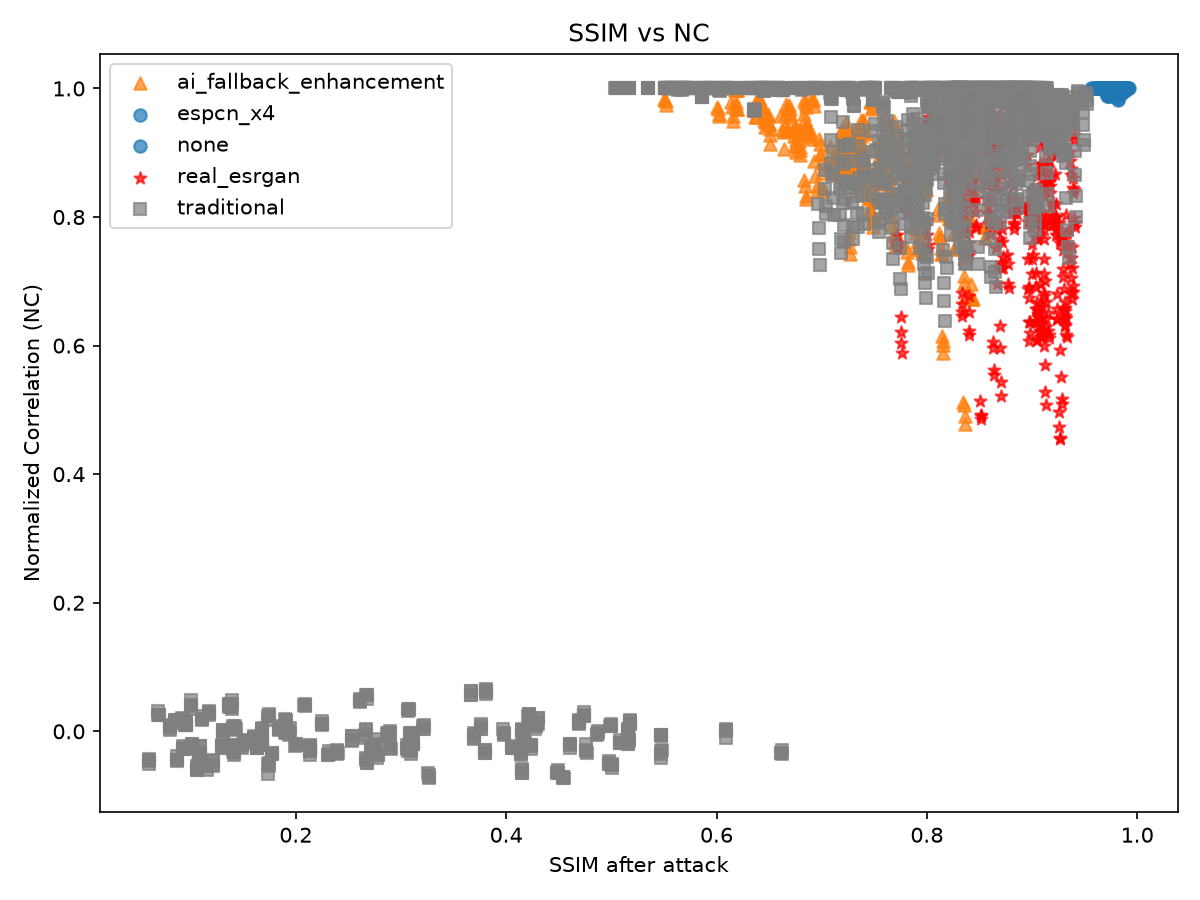
\includegraphics[width=\columnwidth]{figures/ssim_vs_nc.png}
\caption{SSIM vs.\ NC per attacked image. Real-ESRGAN occupies a
high-SSIM, low-NC region unreachable by any classical attack; ESPCN
clusters near $\mathrm{NC}=1.0$ at high SSIM.}
\label{fig:asymmetry}
\end{figure}

\subsection{The Quality--Watermark Asymmetry}
Figure~\ref{fig:asymmetry} shows the central observation. Every
classical attack that reduces NC also reduces SSIM: watermark damage is
coupled to visible quality damage. Real-ESRGAN decouples them, occupying
a high-quality, low-detection region that no classical attack reaches.
Operationally, a content owner monitoring watermark integrity would
observe degraded detection with no visible indication that the image had
been modified --- a qualitatively distinct threat from classical attacks.

\subsection{Embedding Strength Does Not Restore Robustness}
\begin{table}[t]
\caption{Mean NC under Real-ESRGAN by embedding strength $\alpha$,
standard pair $(4,1)/(1,4)$, averaged across 100 images.}
\label{tab:alpha_main}
\centering
\begin{tabular}{ccc}
\toprule
$\alpha$ & NC (Real-ESRGAN) & SSIM \\
\midrule
0.05 & 0.787 & 0.907 \\
0.10 & 0.797 & 0.906 \\
0.20 & 0.815 & 0.906 \\
0.30 & 0.832 & 0.905 \\
\bottomrule
\end{tabular}
\end{table}
Table~\ref{tab:alpha_main} shows NC improves only marginally as $\alpha$
quadruples from 0.05 to 0.30, while SSIM remains flat. For classical
attacks, stronger embedding produces proportionally better survival;
Real-ESRGAN does not exhibit this behavior, consistent with the model
overwriting DCT coefficient relationships during reconstruction rather
than merely attenuating the embedded signal.

\section{Mechanism and Mitigation}
\label{sec:analysis}

\subsection{DCT Coefficient Damage Profiles}
\begin{figure}[t]
\centering
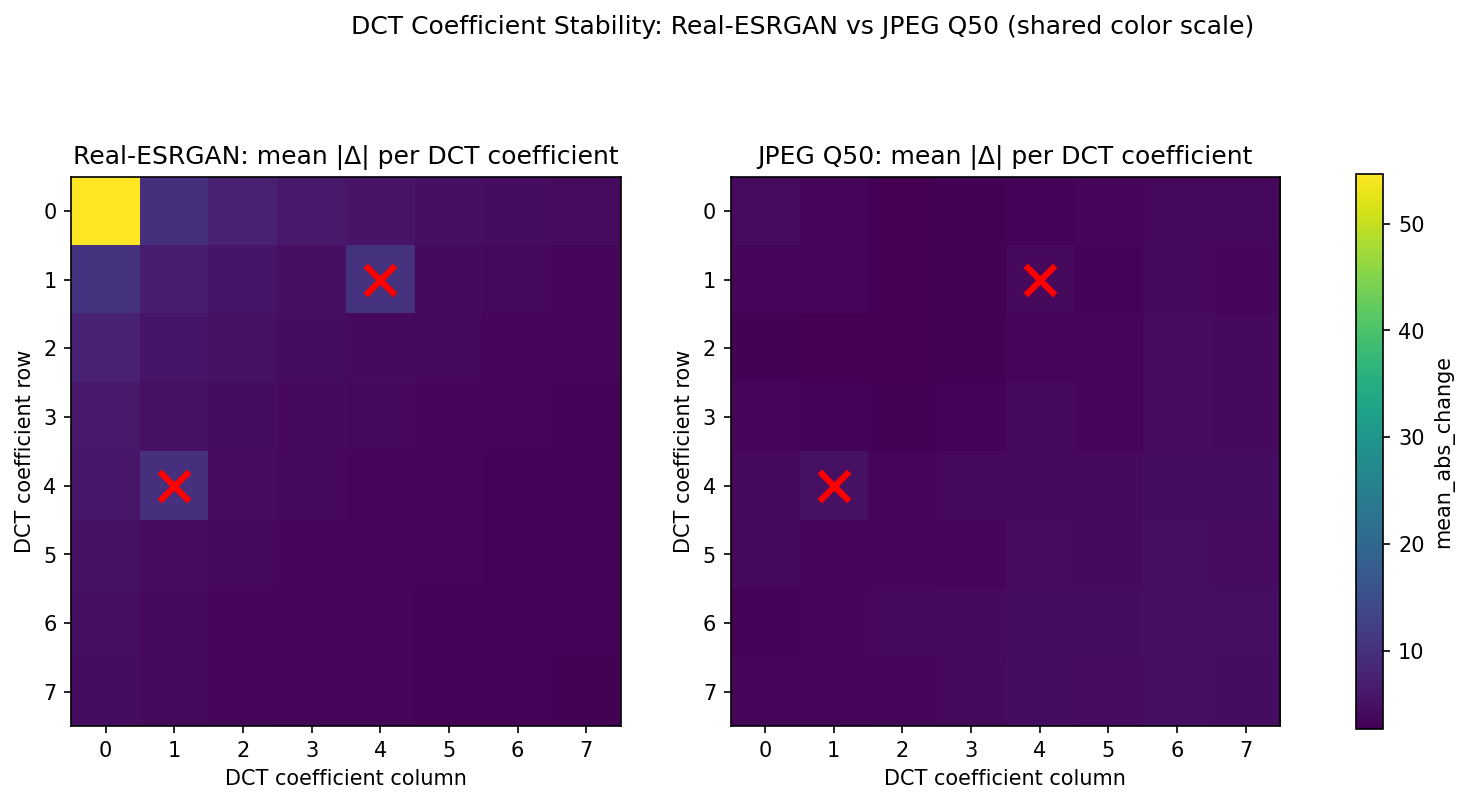
\includegraphics[width=\columnwidth]{figures/dct_stability_comparison.png}
\caption{Mean absolute DCT coefficient perturbation per position for
Real-ESRGAN (left) and JPEG-Q50 (right) across 102,400 blocks, shared
color scale. Real-ESRGAN concentrates damage in the DC coefficient;
JPEG distributes damage nearly uniformly. Baseline embedding positions
$(4,1)$ and $(1,4)$ are marked.}
\label{fig:heatmap}
\end{figure}

Figure~\ref{fig:heatmap} shows mean absolute perturbation per DCT
position. Real-ESRGAN concentrates damage almost entirely in the DC
coefficient at $(0,0)$, with mean perturbation roughly 5 to 14 times
greater than any other position, and elevated perturbation extending
into the low- and mid-frequency region. This pattern is consistent with
the learned reconstruction re-rendering local luminance statistics; it
cannot be attributed to resampling, since ESPCN shares that pipeline and
leaves extraction nearly perfect. JPEG-Q50 distributes damage across all
64 positions in a narrow range with mild elevation at higher frequencies,
consistent with its quantization table design.

The two profiles are strongly anti-complementary: Spearman rank
correlation between the per-position ESRGAN and JPEG damage profiles is
$\rho = -0.716$ ($p < 10^{-10}$), and between the ESRGAN damage profile
and the JPEG quantization step-size vector is $\rho = -0.907$
($p < 10^{-25}$). Positions most damaged by ESRGAN tend to be positions
least damaged by JPEG, and vice versa. This anti-complementarity means
that for any given pair $(r_1,c_1)/(r_2,c_2)$, improving robustness to
one attack by choosing positions where it causes less relative damage
tends to hurt robustness to the other attack.

The classical embedding positions $(4,1)$ and $(1,4)$ sit in a
mid-frequency zone where Real-ESRGAN's perturbation is elevated relative
to the most stable high-frequency corner positions. The
coefficient-selection assumptions inherited from the compression era do
not transfer to the enhancement threat.

\subsection{Exhaustive Pair Search and Pareto Frontier}

To characterize the structure of the ESRGAN/JPEG tradeoff, we compute
robustness scores for all 1,953 valid coefficient pairs derived from the
upper-left $7\times7$ submatrix of the DCT block. For each pair, an
E-score summarizes predicted ESRGAN stability (based on the damage
profile) and a J-score summarizes predicted JPEG robustness (based on
the JPEG quantization table). The Pareto frontier --- pairs no other
configuration dominates on both objectives simultaneously --- contains
37 pairs out of 1,953. The standard baseline pair $(4,1)/(1,4)$ lies
off the Pareto frontier (E-score $= 0.028$, J-score $= 0.877$),
confirming it is not optimal under either attack in isolation or their
combination.

\begin{figure}[t]
\centering
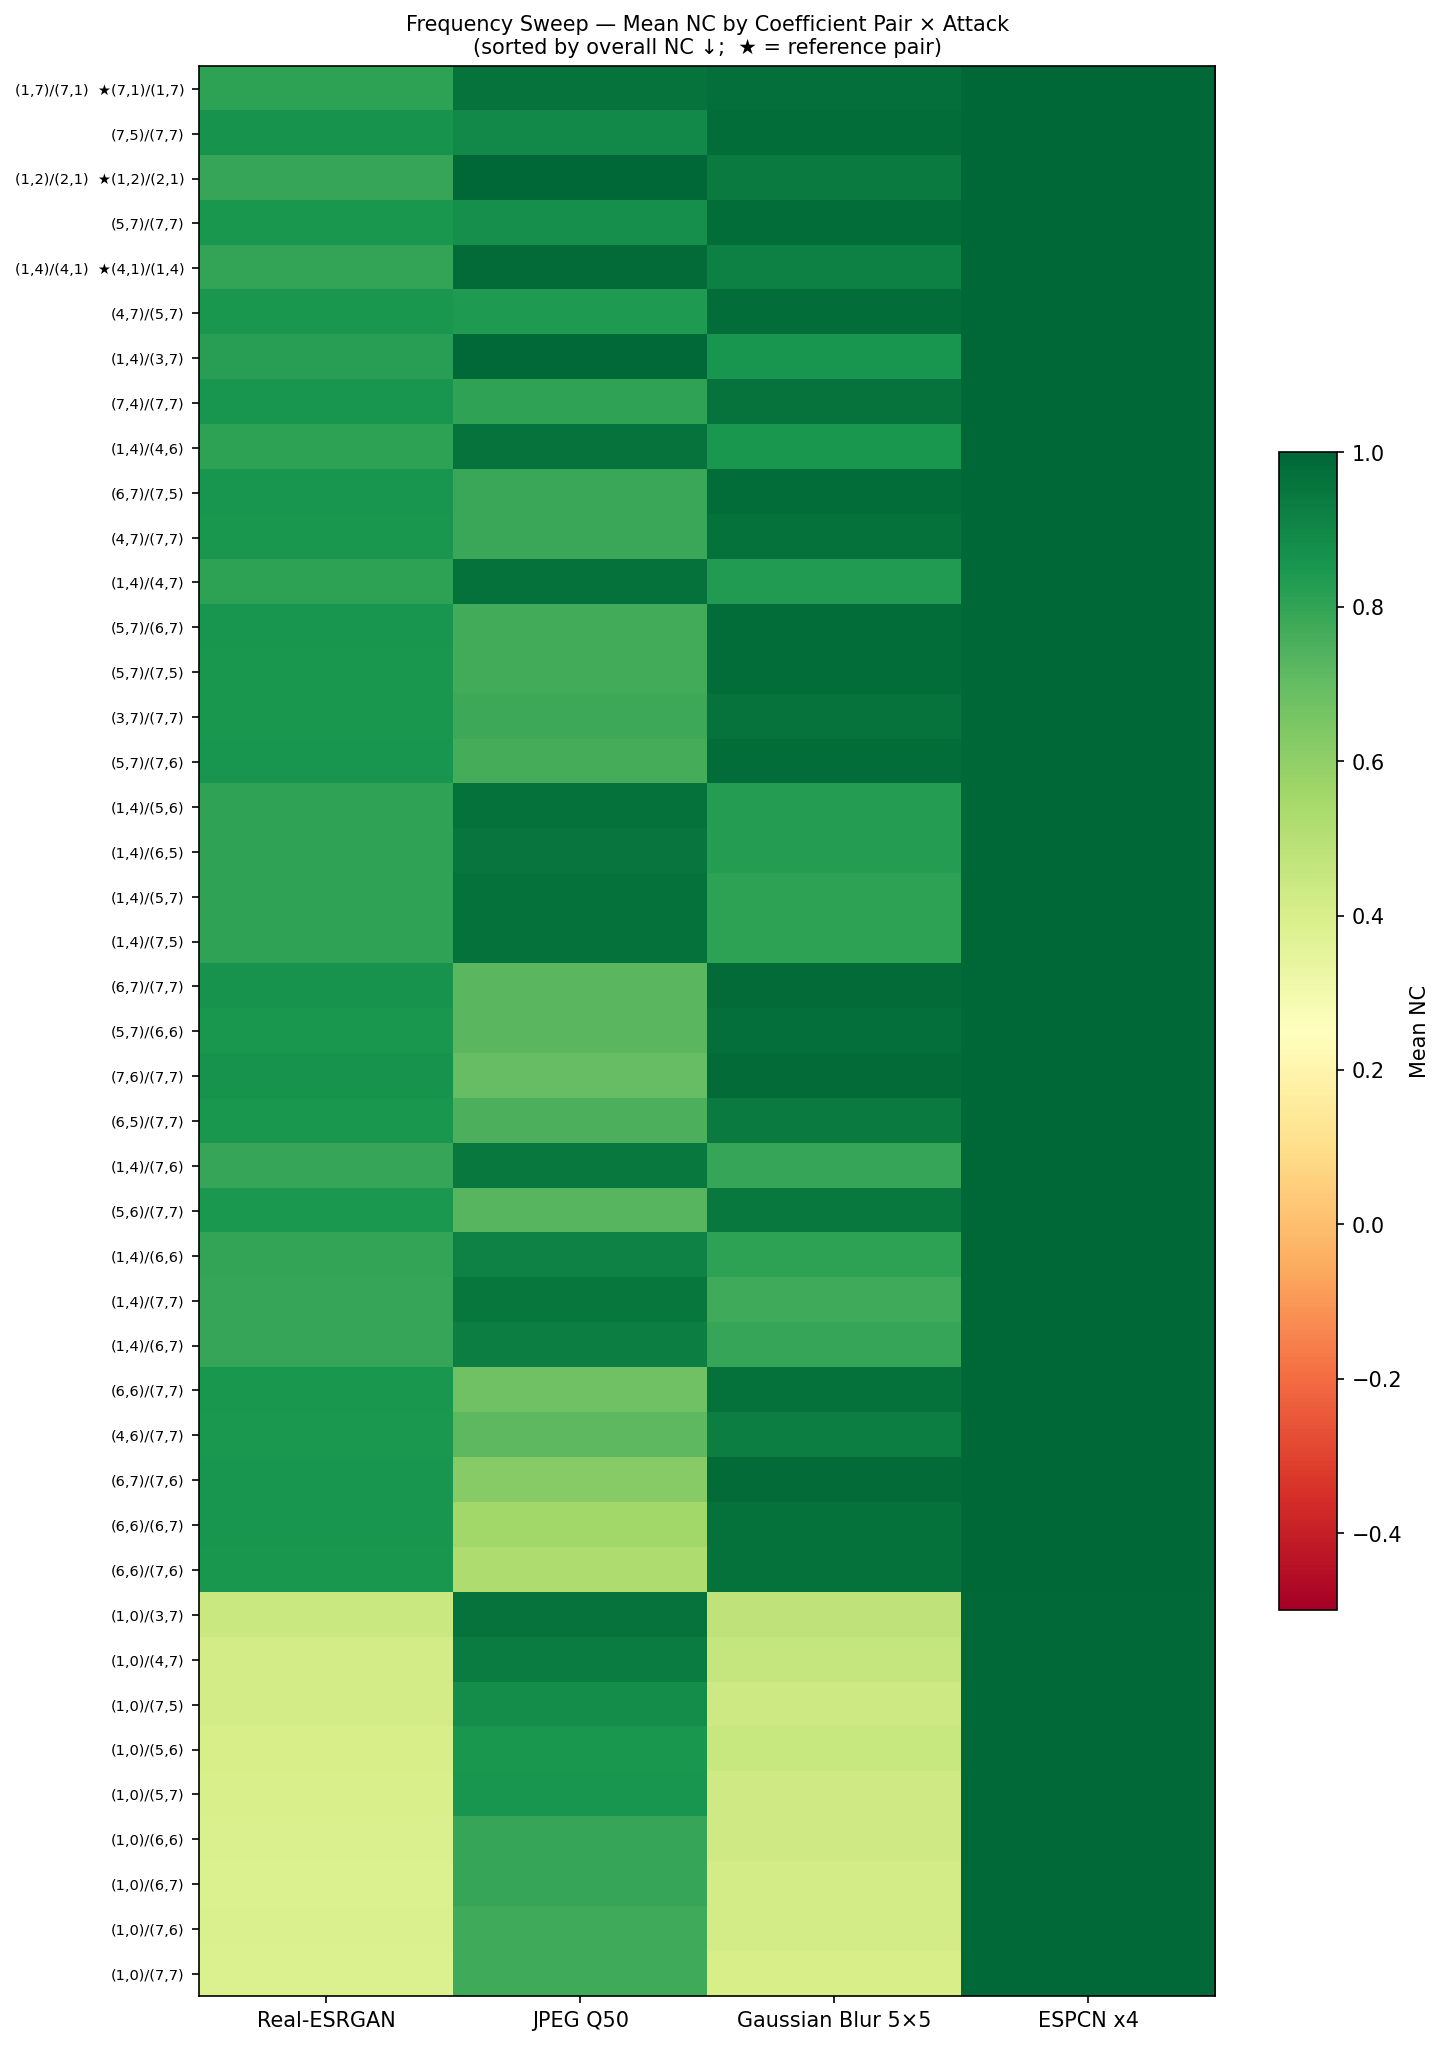
\includegraphics[width=\columnwidth]{figures/frequency_sweep_heatmap.png}
\caption{Real-ESRGAN NC vs.\ JPEG-Q50 NC per coefficient pair. The
Pareto frontier (upper-right boundary) shows no pair simultaneously
maximizes both. Pairs anchored near the high-frequency corner $(7,7)$
achieve highest ESRGAN NC; pairs in the mid-frequency band achieve
highest JPEG NC.}
\label{fig:pareto}
\end{figure}

The anti-complementarity of the damage profiles is directly reflected in
the Pareto plot (Figure~\ref{fig:pareto}): the ESRGAN NC and JPEG NC of
individual pairs are negatively correlated (Spearman $\rho = -0.488$,
$p < 0.001$) across the 43 screened pairs. No pair improves against both
attacks simultaneously relative to the baseline.

\subsection{Three-Pair Full Validation}

We select three pairs spanning the Pareto frontier for end-to-end
validation: the standard pair $(4,1)/(1,4)$, the analytically
Pareto-optimal pair $(2,3)/(3,2)$ (highest combined E+J score among the
37 Pareto-optimal pairs), and the high-frequency pair $(7,5)/(7,7)$
(highest predicted ESRGAN robustness). Each pair is evaluated across all
100 images at all four $\alpha$ values under four attack conditions.
Table~\ref{tab:pairs} shows results at $\alpha=0.10$.

\begin{table}[t]
\caption{Mean NC $\pm$ standard deviation at $\alpha=0.10$ across 100
images for three coefficient pairs under four attack conditions.
All pairwise NC differences across all attack/pair combinations are
statistically significant after BH--FDR correction except no-attack
comparisons ($p < 10^{-12}$ or n.s.\ as indicated).}
\label{tab:pairs}
\centering
\begin{tabular}{lccc}
\toprule
Attack & Standard & Balanced & HF \\
       & $(4,1)/(1,4)$ & $(2,3)/(3,2)$ & $(7,5)/(7,7)$ \\
\midrule
No attack      & $0.9997 \pm 0.000$ & $0.9997 \pm 0.000$ & $1.000 \pm 0.000$ \\
Real-ESRGAN    & $0.783 \pm 0.124$ & $0.683 \pm 0.139$   & $0.831 \pm 0.109$ \\
JPEG-Q50       & $0.995 \pm 0.004$ & $0.998 \pm 0.001$   & $0.902 \pm 0.018$ \\
Gaussian blur  & $0.910 \pm 0.013$ & $0.933 \pm 0.011$   & $0.977 \pm 0.005$ \\
\midrule
PSNR (dB)      & $40.6$ & $40.9$ & $43.9$ \\
\bottomrule
\end{tabular}
\end{table}

\textbf{Real-ESRGAN.} The three pairs rank HF $>$ Standard $>$ Balanced.
The balanced pair (analytically Pareto-optimal) achieves NC of 0.683
under Real-ESRGAN, which is 0.100 NC points below the standard pair
(Wilcoxon, BH-adj.\ $p < 10^{-17}$, Cohen's $d = -1.45$; balanced
NC~$<$~standard NC in 96--100\% of images depending on $\alpha$). The
HF pair achieves NC of 0.831, 0.048 above standard ($p < 10^{-13}$,
$d = 0.89$). These differences are stable across all four embedding
strengths: the balanced--standard ESRGAN gap ranges from $-0.100$ to
$-0.101$ over $\alpha \in \{0.05, 0.10, 0.20, 0.30\}$.

\textbf{JPEG-Q50.} The ordering reverses: Balanced ($0.998$) $>$ Standard
($0.995$) $\gg$ HF ($0.902$). The HF pair suffers a large JPEG regression
($\Delta\mathrm{NC} = -0.094$ vs.\ standard, $p < 10^{-17}$).

\textbf{Gaussian blur.} Ordering follows ESRGAN: HF ($0.977$) $>$
Balanced ($0.933$) $>$ Standard ($0.910$); all differences are large and
highly significant.

\textbf{Imperceptibility.} The balanced pair achieves higher PSNR
($+0.30$\,dB at $\alpha=0.10$), and the HF pair achieves substantially
higher PSNR ($+3.3$\,dB), eliminating below-threshold imperceptibility
failures present in the standard pair.

\textbf{Key finding.} No pair simultaneously achieves the highest NC
across all attacks. The analytical Pareto ranking is not preserved in
end-to-end evaluation: the pair predicted to be the best combined
choice (balanced, $(2,3)/(3,2)$) achieves the lowest Real-ESRGAN NC of
the three. Embedding position selection offers attack-aware partial
mitigation, but the ESRGAN/JPEG tradeoff cannot be resolved within this
scheme.

\subsection{Stability of the Anti-Complementarity Across Embedding Strengths}

A key question is whether the ESRGAN/JPEG anti-complementarity depends
on the embedding strength $\alpha$ --- for example, whether stronger
embedding can shift which positions are most vulnerable. We measure the
per-position ESRGAN and JPEG DCT damage profiles at all four $\alpha$
values and compute cross-attack Spearman correlations and cross-$\alpha$
rank stability for the standard pair.

The ESRGAN/JPEG profile anti-complementarity is essentially constant
across $\alpha$: $\rho$ ranges from $-0.716$ at $\alpha=0.05$ to
$-0.706$ at $\alpha=0.30$, a total range of 0.010 over a $6\times$ span
of embedding strength. The rank ordering of all 64 DCT positions by
damage magnitude is also stable: Jaccard similarity of the top-10
most-damaged positions is 1.0 for all cross-$\alpha$ comparisons, for
both ESRGAN and JPEG independently. This indicates the anti-complementarity
is a structural property of the two attack types, not of the embedding
strength. Similarly, Real-ESRGAN damage isotropy (Spearman $r$ between
damage at symmetric DCT positions) is stable at $r \approx 0.989$
across all tested $\alpha$ values.

\subsection{Symmetry Analysis}

Symmetric coefficient pairs ($(r,c)/(c,r)$) achieve mean NC of 0.821
under Real-ESRGAN versus 0.689 for asymmetric pairs across the 43-pair
screening set (Table~\ref{tab:symmetry}), disconfirming the hypothesis
that coordinate symmetry contributes to Real-ESRGAN vulnerability.

\begin{table}[t]
\caption{Mean NC by coefficient-pair symmetry category (43-pair
screening set, $\alpha=0.1$, 20-image subset).}
\label{tab:symmetry}
\centering
\begin{tabular}{lcccc}
\toprule
Category & ESRGAN & JPEG & Blur & Overall \\
\midrule
Symmetric      & 0.821 & 0.866 & 0.959 & 0.911 \\
Near-symmetric & 0.856 & 0.721 & 0.976 & 0.888 \\
Asymmetric     & 0.689 & 0.868 & 0.735 & 0.822 \\
\bottomrule
\end{tabular}
\end{table}

\subsection{Subband Selection Does Not Help}
As a supplementary comparison, we evaluated a DWT-SVD scheme embedding
in the HH subband at matched imperceptibility (47.7 vs.\ 48.0\,dB
PSNR). It achieves NC of only 0.18 under Gaussian blur and JPEG-Q50 and
0.29 under Real-ESRGAN --- near-chance extraction under attacks
the DWT-DCT-LL scheme survives at 0.93, 0.98, and 0.75 respectively.
Moving embedding energy to high-frequency subbands is not a viable
escape from the enhancement vulnerability.

\subsection{Limitations}
Our evaluation covers two enhancement architectures; the threat is
architecture-specific (ESPCN vs.\ Real-ESRGAN), and characterizing
enhancement as a general attack category requires evidence across a
broader model family. All headline results are for one classical scheme
(DWT-DCT with ordering-based bit encoding); generalization to other
classical schemes remains to be established. The Pareto analysis uses
proxy scores (damage-profile-based E-score and J-score) rather than
end-to-end NC; the three-pair full validation confirms that the proxy
ranking does not reliably predict end-to-end robustness ordering: the
highest-combined-score pair achieves the lowest empirical ESRGAN NC
among the three candidates tested.

\section{Conclusion}
\label{sec:conclusion}

We investigated whether AI-based image enhancement violates the
quality--attack tradeoff underlying classical watermark robustness
evaluation, and found that it can: Real-ESRGAN degrades DWT-DCT
watermark recovery to NC $= 0.795$ while producing the highest perceptual
quality of any attack tested, while ESPCN --- sharing the identical
resampling pipeline --- leaves watermarks intact. The mechanism is a
DC-concentrated perturbation profile fundamentally unlike JPEG's uniform
profile, with strongly anti-complementary position rankings
($\rho \approx -0.7$ to $-0.9$). An exhaustive search over 1,953
coefficient pairs confirms that this anti-complementarity is reflected
in end-to-end NC: no pair simultaneously maximizes Real-ESRGAN and JPEG
robustness. Three-pair head-to-head validation on 100 images at four
embedding strengths finds large, statistically significant,
attack-dependent NC differences ($p < 10^{-12}$ after BH--FDR correction),
with the ESRGAN/JPEG ranking reversing between attacks. The
anti-complementarity is stable across embedding strengths $\alpha \in
\{0.05, 0.10, 0.20, 0.30\}$ ($\rho$ range $\leq 0.010$; position rank
order perfectly preserved), indicating it is a structural property of
the two attack types.

Content owners relying on DWT-DCT watermarking should be aware that
consumer enhancement tools can silently degrade watermark integrity.
Attack-aware coefficient selection offers partial mitigation: the
high-frequency pair $(7,5)/(7,7)$ improves Real-ESRGAN NC from 0.795 to
0.831 and eliminates imperceptibility failures at the cost of JPEG NC
(0.996 to 0.902), while the balanced pair $(2,3)/(3,2)$ favors JPEG
robustness but performs below the standard pair under Real-ESRGAN.
Future work should investigate content-adaptive strategies that jointly
optimize coefficient selection and embedding against both attack types,
and should extend the evaluation to a broader family of enhancement
models.

\section*{Acknowledgment}
The author used Claude (Anthropic) as an AI coding assistant for
pipeline implementation. All experimental design, analysis, and writing
are the author's own work.

\bibliographystyle{IEEEtran}
\bibliography{references_revised}

\end{document}
